\documentclass[preprint]{sigplanconf}
\usepackage[utf8]{inputenc}
\usepackage{graphicx,tikz}
\usepackage{color}
\usepackage{amsfonts,amsmath,amsbsy,amsthm,amssymb}
\usepackage[final,bookmarks,colorlinks,linktocpage,linkcolor=black,citecolor=black,urlcolor=blue]{hyperref}
\usepackage{tikz-qtree}
\usepackage{url}
\usepackage{xspace}
\usepackage{listings}
\usepackage{decade}
\usepackage{mathpartir}
\usepackage{xargs}
\usepackage{turnstile}
\usepackage{pifont}
\usepackage{breqn}
\usepackage{wasysym}
\usepackage{mathtools}

\bibliographystyle{abbrv}
\sloppy

%%%%%%%%%%%%%%%%%%%%%%% Commands %%%%%%%%%%%%%%%%%%%%%%%%

\lstset{
  basicstyle=\footnotesize\ttfamily,
  columns=fullflexible,
  language=rml,
  showstringspaces=false,
  keywordstyle={\bfseries\color{blue}}
}

\newenvironment{example}%
{\vspace{1em}
{\noindent
 \bf Example.}
 \it}%
{\vspace{1em}}

\newcommand{\ie}{i.e.,\xspace}
\newcommand{\eg}{e.g.,\xspace}
\newcommand{\tight}{{\tt{tight}}\xspace}
\newcommand{\loose}{{\tt{loose}}\xspace}
\renewcommand{\partial}{{\tt{partial}}\xspace}
\newcommand{\causal}{{\tt{causal}}\xspace}
\newcommand{\local}{{\tt{local}}\xspace}
\newcommand{\globl}{{\tt{global}}\xspace}
\newcommand{\group}{{\tt{group}}\xspace}
\newcommand{\event}{{\tt{event}}\xspace}

\newcommand{\alt}{\;|\;}

\newcommand{\langname}[1]{{#1}\xspace}
\newcommand{\Antescofo}{\langname{Antescofo}}
\newcommand{\ReactiveML}{\langname{ReactiveML}}
\newcommand{\rml}{\ReactiveML}
\newcommand{\Ocaml}{\langname{OCaml}}
\newcommand{\Haskell}{\langname{Haskell}}
\newcommand{\Lustre}{\langname{Lustre}}
\newcommand{\Esterel}{\langname{Esterel}}

\renewcommand{\k}[1]{{\bf \color{blue}{\ttfamily #1}}}
\newcommand{\f}[1]{{\footnotesize{\ensuremath{\mathtt{#1}}}}}
\newcommand{\ti}[1]{{\tiny{\ensuremath{\mathtt{#1}}}}}
\renewcommand{\ll}[1]{{{\ensuremath{\mathtt{#1}}}}}
\newcommand{\p}{\textbar \xspace}
\newcommand{\m}[1]{{{\mbox{\emph{#1}}}}}
\renewcommand{\l}[1]{\lstinline[basicstyle=\normalsize\ttfamily]{#1}}




\newcommand{\M}{\mathcal{M}}
\newcommand{\E}{\mathcal{E}}
\newcommand{\Extract}{\m{\textup{Extract}}}
\newcommand{\Split}{\m{\textup{Split}}}
\newcommand{\Slice}{\m{\textup{Slice}}}
\newcommand{\seq}{\ensuremath\mathit{seq}}

% %%%%%%%%%%%%%%%%%%%%% vdash for inference rules %%%%%%%%%%%%%%%%%%%%%%%%%%

\newcommand{\mvdash}[1]{\mbox{\setlength{\unitlength}{0.1em}%
 \begin{picture}(27,10)%
 \put(0,-3){\line(0,1){11}}%
 \put(0,3){\line(1,0){27}}%
\put(11,8){%
  \makebox(0,0)[t]{\tiny #1}}%
 \end{picture}%
 }%
 }

\newcommand{\svdash}[1]{\mbox{\setlength{\unitlength}{0.1em}%
 \begin{picture}(20,10)%
 \put(0,-3){\line(0,1){11}}%
 \put(0,3){\line(1,0){20}}%
\put(11,8){%
  \makebox(0,0)[t]{\tiny #1}}%
 \end{picture}%
 }%
 }

%%%%% Inference Macros %%%%%
%% \newcommand{\context}{i,\delta}
%% \newcommand{\rularrow}[4]{{#1}~\mvdash{#2}~{#3}\rightarrow{#4}}
%% \newcommand{\ruliter}[4]{{#1}~\mvdash{#2}~{#3}\Rightarrow{#4}}
%% \newcommandx*{\rdetect}[4][2=~~detected]{\rularrow{#1}{#2}{#3}{#4}}
%% \newcommandx*{\rmissed}[4][2=missed]{\rularrow{#1}{#2}{#3}{#4}}
%% \newcommandx*{\rgeneric}[4][2=~generic]{\rularrow{#1}{#2}{#3}{#4}}
%% \newcommandx*{\ritergeneric}[4][2=~generic]{\ruliter{#1}{#2}{#3}{#4}}
%% \newcommandx*{\riterdetect}[4][2=~~detected]{\ruliter{#1}{#2}{#3}{#4}}
%% \newcommandx*{\ritermissed}[4][2=missed]{\ruliter{#1}{#2}{#3}{#4}}
%% \newcommand{\rexec}[3]{#1 ~\svdash{exec\phantom{d}}~#2\rightarrow#3}
\newcommand{\context}{i,\delta}

% Version de Marc
%% \newcommand{\rularrow}[4]
%% {{#1}\stackrel{\mathit{#2}}{\vdash}{#3}\rightarrow{#4}}
%% \newcommand{\ruliter}[4]
%%            {{#1}\stackrel{\mathit{#2}}{\vdash}{#3}\Rightarrow{#4}}


\newcommand{\rularrow}[4]{{#1}~\sststile{}{\mathit{#2}}~{#3}\rightarrow{#4}}
\newcommand{\ruliter}[4]{{#1}~\sststile{}{\mathit{#2}}~{#3}\Rightarrow{#4}}

%% \newcommand{\rularrow}[4]{{#1}~\vdash~{#3}\xrightarrow{ \mbox{\tiny $\mathit{#2}$}}{#4}}
%% \newcommand{\ruliter}[4]{{#1}~\vdash~{#3}\xRightarrow{\mathit{#2}}{#4}}


\newcommandx*{\rdetect}[4][2=detected]{\rularrow{#1}{#2}{#3}{#4}}
\newcommandx*{\rmissed}[4][2=missed]{\rularrow{#1}{#2}{#3}{#4}}
\newcommandx*{\rgeneric}[4][2=generic]{\rularrow{#1}{#2}{#3}{#4}}
\newcommandx*{\ritergeneric}[4][2=generic]{\ruliter{#1}{#2}{#3}{#4}}
\newcommandx*{\riterdetect}[4][2=detected]{\ruliter{#1}{#2}{#3}{#4}}
\newcommandx*{\ritermissed}[4][2=missed]{\ruliter{#1}{#2}{#3}{#4}}
%% \newcommand{\rexec}[3]
%%   {{#1}\stackrel{\mathit{exec}}{\vdash}{#2} \rightarrow {#3}}

\newcommandx*{\rexec}[4][2=exec]{\rularrow{#1}{#2}{#3}{#4}}
\newcommandx*{\riterexec}[4][2=exec]{\ruliter{#1}{#2}{#3}{#4}}

%%%%%%%%%%%%%%%%%%%%%%%%
% Liens vers le code
\newcommand{\webdir}{https://sites.google.com/site/reactiveasco/}
\newcommand{\rmldev}[1]{{\href{\webdir#1}{\ensuremath{^\bigstar}}}}
\newcommand{\video}[1]{{\href{\webdir videos/#1}{\twonotes}}}

%annexes
\newcommand{\refappendix}[1]{
\ifthenelse{\boolean{extended}}
{\ref{#1}}
{\ref{#1} of the extended version}}

%%%%%%%%%%%%%%%%%%%%%%%%
% add personnal comments
\newcommand{\Marc}[1]{{\sl \textcolor{red}{\textbf{MP:} {#1}\xspace}}}
%\renewcommand{\Marc}[1]{}
\newcommand{\Florent}[1]{[{\sl\small \textcolor{red}{\textbf{F:} #1}}]\xspace}
%\newcommand{\Florent}[1]{}
\newcommand{\Guillaume}[1]{[{\sl\small \textcolor{green}{\textbf{G:} #1}}]\xspace}


\title{A Synchronous Embedding of Antescofo, a Domain-Specific Language for Interactive Mixed Music}


\authorinfo{Guillaume Baudart}
          {\'Ecole normale sup\'erieure de Cachan \\
           Antenne de Bretagne\\
          Campus de Ker-Lann, 35170 Bruz}
          {Guillaume.Baudart@ens-cachan.org}

\authorinfo{Louis Mandel
            \and Marc Pouzet}
           {DI, \'Ecole normale sup\'erieure \\
            45 rue d'Ulm, 75230 Paris}
           {Firstname.Name@ens.fr}

\begin{document}
\maketitle

\section{A Language for Mixed Music}
\label{sec:antescofo}

We now describe the kernel of the \Antescofo language, a language
dedicated to the writing of mixed music
scores~\cite{echeveste2012antescofo}. This language was developed as a
language for coordinating events performed by humans and electronic
actions controlled by a computer.  It allows a composer to specify
both electronic and instrumental parts in the same
score. Figure~\ref{fig:asco_score} shows a simple example of one such
score (the symbol~\video{} indicates a link to a demonstration video
available online).

The language permits expressing delays relative to a tempo expressed
in beats per minute ($\m{bpm}$). For instance, a duration of~$1.0$
means ${1.0\ \m{beat}}$. During a performance, the listening machine
estimates both the position in the score and the tempo of the
performer. This allows the sequencer to follow the speed of the
performer as would a trained musician. Indeed, the tempo is not
estimated from the last duration alone but rather from all durations
detected since the beginning of the performance. In this way, the
listening machine adds some inertia to tempo changes which corresponds
to the real behavior of musicians playing
together~\cite{cont2008antescofo}.  This feature explains some of the
success of \Antescofo with composers, as synchronizing different parts
using a common tempo is standard practice when writing polyphonic
music (in many other environments for mixed music, delays can only be
expressed in milliseconds).




\subsection{The Core Language}
\label{sec:language}

The main idea is to bind electronic actions to instrumental
events. During a performance, actions related to an instrumental event
are executed when the event is detected. Thus, a~\emph{score} is a
sequence of instrumental events and for each such event an associated
sequence of electronic action.  It is described by the following
grammar (the empty sequence is denoted~$\varepsilon$).
%
\[
\begin{array}{rcl}
  \m{score} &::=& \varepsilon \alt
                  (\m{event} :  \m{seq}) \; \m{score}  \\
  \m{event} &::=& \event \; i \; t\\
  \m{seq} &::=& \varepsilon \alt (\delta \ ae) \; \m{seq} \\
  ae &::=& \m{action} \alt \m{group} \\
  \m{group} &::=& \group \; \m{synchro} \; \m{error} \; \m{seq} \\
  \m{synchro} &::=&  \tight \alt \loose \\
  \m{error} &::=& \local \alt \globl \alt \partial \alt \causal\\
\end{array}
\]
%
An instrumental event (e.g., a note, chord, trill, etc.) is denoted
by~$\event \; i \; t$, where~$i \in \mathbb{N}$ is the index of an
event in the score and~$t \in \mathbb{Q}$ its duration relative to the
tempo.  Indeed, for the sequencer, instrumental events are only
triggers for electronic actions. Therefore, the only useful
information is the position and the duration of an event. An
electronic action~($ae$) is either an atomic action taken from a
finite set ($\m{action} \in \mathbb{A}$) or a group of electronic
actions.  A group is a sequence of electronic actions characterized by
a synchronization strategy (described in
Section~\ref{sec:ante_synchro}) and an error handling strategy
(described in Section~\ref{sec:ante_error}).  A sequence ($\seq$) is a
list of pairs, each associating an electronic action ($ae$) with a
delay ($\delta$) relative to the tempo ($\delta \in \mathbb{Q}$).

\begin{figure}
\centering
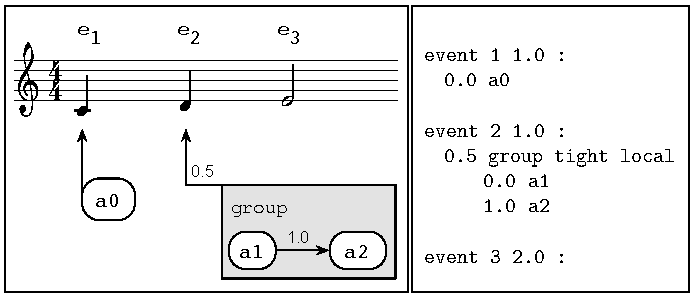
\includegraphics[scale = 0.71]{asco_score.pdf}
\caption{%A first \Antescofo score.  On the left is a graphical
  Representation of an \Antescofo{} score; on the right its textual
  representation.  Musical notes correspond to the musician's part and
  the rest to electronic actions.\video{presentation}}
\label{fig:asco_score}
\end{figure}

The most basic actions in a score, called \emph{atomic actions}, are
simple control messages destined for the audio environment (e.g.,
Max/MSP).  Each is bound to an instrumental event, the
\emph{triggering event}, and characterized by a delay. When the
listening machine detects the triggering event, the sequencer waits
for the specified delay and then sends the corresponding control
message.  In the example of Figure~\ref{fig:asco_score}, action~$a_0$
is bound to the first note with a delay of~$0.0$. Thus, when the first
note is detected, the message~$a_0$ is sent immediately.

Atomic actions can be grouped into control structures called
\emph{groups}. Like an atomic action, a group is triggered by an
instrumental event and characterized by a delay. When the triggering
event is detected, the sequencer waits for the corresponding delay and
then launches the actions contained in the body of the group. In the
example, a group is bound to the second instrumental event with a
delay of~${0.5 \; \m{beat}}$. When this event is detected, the
sequencer waits~${0.5 \; \m{beat}}$ and then launches action~$a_1$,
after another delay of~${1.0 \; \m{beat}}$, the message~$a_2$ is sent.
Groups can be nested arbitrarily. Actions contained in a nested group
are executed in parallel with the actions following them in the
embedding group, not in sequence. An electronic voice can be split in
two parallel voices which can in turn be split and so on. Thus, a
score can faithfully capture the complexity of a musical piece.

There are two kinds of parallelism in the language. First, two
sequences bound to different instrumental events are executed in
parallel. Second, a nested group inside a sequence is executed in
parallel with the rest of the sequence. Note that when two sequences
are executed in parallel, it is important that they share the same
global time: the time of the performance.  That is, they must be
synchronous!  Otherwise the performance would not reflect the musical
score.  To this fundamental similarity with typical synchronous
languages, \Antescofo{} adds two major original features:
synchronization and error handling strategies.

\subsection{Synchronization Strategies}
\label{sec:ante_synchro}
Groups are characterized by two attributes (see \cite{ContEGJ12icmc}).
The first one defines a synchronization strategy. A composer is
allowed to specify how actions contained in a group will synchronize
with instrumental events that occur during the execution of the
group. There are several ways to achieve this synchronization
depending on the musical context. Currently, the language proposes two
distinct modes of synchronization:

\paragraph{The strategy {\tt loose}}
Once a group is launched, delays are computed according to the current
tempo value, regardless of instrumental events that may occur during
its execution.  Due to the inertia of the tempo inference, an
electronic action contained in such a group and an instrumental event
that seems to be simultaneous in the score may be desynchronized
during the performance.  Indeed, a performer may accelerate or
decelerate between two events. Typically, this strategy is used in
those parts of a score where a performer follows the electronic
voices.

\paragraph{The strategy {\tt tight}}
In this strategy, every action of a group is triggered by the most
recent corresponding instrumental event.  In the example of
Figure~\ref{fig:asco_score}, the first group has a synchronization
attribute set to \tight.  Thus, although the entire group is bound to
the second instrumental event, action $a_2$ will be triggered
by~$e_3$. Here, the nearest event is computed with respect to the
ideal timing of the score regardless of tempo changes. This strategy
is ideal when the electronic voice must accompany the interpreter's
voice.

\subsection{Error Handling Strategies}
\label{sec:ante_error}
\Antescofo is designed to accompany real musicians and, thus, errors
may sometimes occur. By error we mean an instrumental event which is
expected and missing, either because it was not played by the musician
or not detected by the listening machine.  The second attribute of a
group defines the error handling strategy which should be taken when
an expected triggering event is absent.  There are several ways to
deal with errors depending on the musical context. Here, we present
four exclusive error handling strategies: \local, \globl, \partial and
\causal. Figure~\ref{fig:error_behaviors} illustrates the four
different behaviors.

The \local and \globl strategies preserve the integrity of a group.
Indeed, if the triggering event is missed, the group is either
completely ignored~(\local) or launched with zero delay~(\globl) as
soon as a later event is detected. In both cases, delays between
actions within the group are unchanged. The group can thus be seen as
a single block with a certain duration.

The other two strategies aim to preserve a simple property: \emph{The
  future of a performance does not depend on past errors}, \ie the
show must go on! When an error occurs, the corresponding group is
split in two parts: actions that should already have been launched
when the error was detected, termed the \emph{past}, and actions that
should occur after the detection, termed the \emph{future}.  The
attributes~\partial and~\causal differ only in their treatment of past
actions. For \causal groups, past atomic actions are launched
immediately. For \partial groups, past atomic actions are simply
discarded. In both cases, future actions are launched as if they were
bound to the next detected event. They are performed as if an error
never occurred.

\begin{figure}
\centering
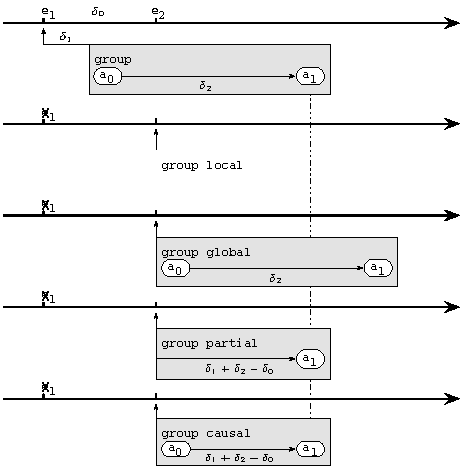
\includegraphics[scale = 1]{error_behaviors.pdf}
\caption{Illustration of the four error handling attributes on a
  simple score (on top). $e_1$ and $e_2$ represent instrumental events. Suppose that $e_1$ is missed and $e_2$ is detected.}
\label{fig:error_behaviors}
\end{figure}



\bibliography{biblio}

\newpage




\end{document}
